%%%%%%%%%%%%%%%%%%%%%%%%%%%%%%%%%%%%%
%%%%% PHYS305 Assignment 7
%%%%% Zachary Martin
%%%%% 13 March 2019
%%%%%%%%%%%%%%%%%%%%%%%%%%%%%%%%%%%%%

\documentclass[aps,prl,twocolumn,superscriptaddress]{revtex4-1}

\usepackage{graphicx}  % this is the up-to-date package for all figures
\graphicspath{{pictures/}} 	% Set Graphics Path
\usepackage{siunitx} % Scientific Notation and Units
\sisetup{separate-uncertainty}
\DeclareSIUnit\celeven{C^{11}}
\DeclareSIUnit\ctwelve{C^{10}}
\usepackage{amsmath, amssymb, gensymb, mathtools, bm, bigints} 	% Mathematical Tools
\usepackage{verbatim}  % for the comment environment
\usepackage{color}
% \usepackage{arydshln} % Dashed lines in table

% For inserting code snippets
\usepackage{listings}
\usepackage{xcolor}
\lstset { %
    language=C++,
    backgroundcolor=\color{black!5}, % set backgroundcolor
    basicstyle=\footnotesize,% basic font setting
}

% Shortcut Commands
\newcommand{\paren}[1]{\left( #1 \right)} 	% Parentheses for complicated expressions
\newcommand{\bparen}[1]{\left[ #1 \right]}	% Bracket parentheses for complicated expressions
\newcommand{\cmod}[1]{\left| #1 \right|}	% Mod or Absolute value

\bibliographystyle{apsrev}

% these are some custom control of the page size and margins
% \topmargin= 0.2in  % these 1st two may be needed for some computers
\textheight=9in
\textwidth=6.5in
% these next two lines give us centered text
\oddsidemargin=0cm
\evensidemargin=0cm

\begin{document}

% Title Contents
\title{PHYS 305 Assignment 7: Numerical Solutions to Differential Equations via Euler and Runge-Kutta Methods.}
\author{Zachary Martin}
\affiliation{University of Hawaii at Manoa}
\date{13 March 2019}

\begin{abstract}
We employ the Euler and Runge-Kutta numerical methods to solve equations of motion for both a system of known analytic solution (a mass on a spring) and a system of unknown analytic solution (large angle pendulum). Using conservation of energy as a measure of accuracy, we find that fourth-order Runge-Kutta methods using step sizes of $dt = \SI{1}{\ms}$ give fractional energy differences below $3*10^{-15}$\% per cycle. We also find that unlike what small angle approximation solutions predict, the period of the pendulum does have a relationship to the initial angle amplitude, and it goes just as we would expect.
\end{abstract}

\maketitle

\section{Introduction and Overview}
An important aspect of physics problems involves solving differential equations. These usually come from the equations of motion of the system. We would like to examine different approximations to solve differential equations via computational methods. The methods involved will be Euler's method and second-order and fourth-order Runge-Kutta method.

\subsection{Mass on a Spring}

\begin{figure}[htbp]
  	\begin{center}
 		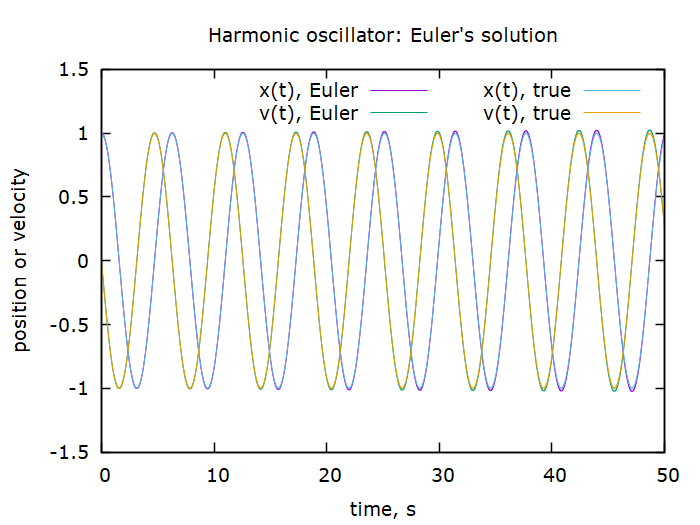
\includegraphics[scale=0.3]{ho1.png}
  		\caption{Simple Harmonic Oscillator solved using Euler's method at step sizes of $\SI{1}{\ms}$. Note that the results are under the true lines. A fit to the numerical results gives the frequency $\omega = \SI{0.999997 \pm 0.000005}{\radian\per\s}$ and a phase $\delta = \SI{0.0009 \pm 0.0001}{\radian}$, which agrees extremely well with the true values of $\omega = \SI{1}{\radian\per\s}$ and $\delta = 0$.}
  		\label{gr:harmosc1}
 	\end{center}
\end{figure}

We start with a simple system for which we know the solution to: a mass on a spring. This system has the equations of motion
\begin{align}
\frac{dx}{dt} &= v \label{eqn:sprx} \\
\frac{dv}{dt} &= -\frac{k}{m} x ~,  \label{eqn:sprv}
\end{align}

where $k$ is the spring constant and $m$ is the mass of the object on the spring. We know that the solution to this is simply
\begin{align}
x(t) &= x_0 \cos (\omega t) \\
v(t) &= v_0 - \omega x_0 \sin (\omega t) ~.   \label{eqn:sprsol}
\end{align}

We can derive the energy at any time $t$ for this system to be
\begin{equation}
E_s = \frac{1}{2}kx^2 + \frac{1}{2}mv^2 ~. \label{eqn:eners} 
\end{equation}

Since energy is conserved, we can assume that the total energy is just the energy of the initial conditions at $x_0, v_0$. Knowing this, we can experiment with different approximation techniques to calculate the solution to the differential equation and compare the results.

\subsection{Large Amplitude Pendulum}
Once we get a grasp of how the approximations work on a system we do know the exact solution to, we can solve another system that we don't know the exact solution to: a large amplitude pendulum. The general equations of motion are
\begin{align}
\frac{d\theta}{dt} = \omega \label{eqn:pend1} \\
\frac{d\omega}{dt} = -\frac{g}{L} \sin \theta \label{eqn:pend2} ~,
\end{align}
where $g$ is the gravitational acceleration and $L$ is the length of the pendulum string. Note that these equations are assuming the pendulum bob is held by an always tight string, or more so a massless rod, so that it falls always a distance $L$ from the pivot point. We can derive that the energy at any time $t$ during the swing will be
\begin{equation}
E_p = \frac{1}{2}m(\omega L)^2 + mgL(1-\cos\theta) \label{eqn:pendener} ~.
\end{equation}
The differential equations have the same exact form as that of a mass on a spring if we apply the small angle approximation and let $\sin \theta = \theta$, for $\theta$ in radians. However, we are more interested in the general case where $\theta$ is chosen freely. Since our variable $\theta$ is inside the sine function, we cannot solve this exactly. It is necessary that we use numerical approximations.

\section{The Computational Problem}

The importance of numerical approximations is evidence for the need of computational methods. We want to solve the equations of motions step by step through time, starting from our initial conditions and working our way through. One method of solving the coupled differential equations like \ref{eqn:sprx} and \ref{eqn:sprv} is called Euler's method. The idea of this method is to approximate each segment as a line, using the slope at each point to move to the next point. Thus, the approximation has the linear form \cite{Euler}
\begin{equation}
y_{i+1}(t+dt) = y_i(t) + \paren{\frac{dy}{dt}}_i (t) dt ~. \label{eqn:euler}
\end{equation}
The method can work, but there are better ways to numerical approximate the solutions. The actual slope from point to another is changing of course, since the solutions are not linear. Euler's method does not account for this change in slope \cite{Laulima}. One way to account for this is to add another term that depends on the midpoint of the steps which will correct for the change in slope. This is the main idea behind the Runge-Kutta method. Since we are only making approximations, there are infinite orders or corrections to make in order to gain an exact solution. We are only interested in second-order (RK2) and fourth-order (RK4) solutions. The RK2 method uses
\begin{align}
y(d+dt) &= y(t) + k_2 \label{eqn:rk2main} \\
k_2 &= dt f( t+\frac{dt}{2}, y(t)+\frac{k_1}{2}) \label{eqn:rk2k2} \\
k_1 &= dt f(t, y(t)) \label{eqn:rk2k1} ~,
\end{align}
where we defined $f(t, y(t)) = \frac{dy}{dt}$. Notice that the correction terms are built upon the ideas from Euler's method.
If we want to go to the fourth order correction, we instead use the equations
\begin{align}
y(t+dt) &= y(t) + k_5 \\
k_5 &= \frac{1}{6} (k_1 + 2k_2 + 2k_3 + k_4) \\
k_1 &= dt f(t, y) \\
k_2 &= dt f( t+\frac{dt}{2}, y(t)+\frac{k_1}{2}) \\
k_3 &= dt f( t+\frac{dt}{2}, y(t)+\frac{k_2}{2}) \\
k_4 &= dt f( t+dt, y(t)+k_3 ) ~.
\end{align}
The equations of motion give us coupled differential equations. Thus, each method will have to be used on each coupled equation and they will build each other up from there.

At each step, we will want to measure how the energy is conserved. If the approximations are correct, we should expect to have constant energy. To measure the fractional difference in the energy per period, we will measure
\begin{equation}
\frac{(dE/E)}{T} = \frac{\cmod{E_t - E}/E}{T} \label{eqn:fracener} ~.
\end{equation}
Here, $E_t$ represents the energy at each step, or each time $t$, and $E$ is the total energy from the initial values. Conservation of energy per period will be our measure of how accurate the approximations are.

Clearly, this is a tedious task. A computer can calculate these approximations for a given step size $dt$ in a short time.

\begin{figure}[htbp]
  	\begin{center}
 		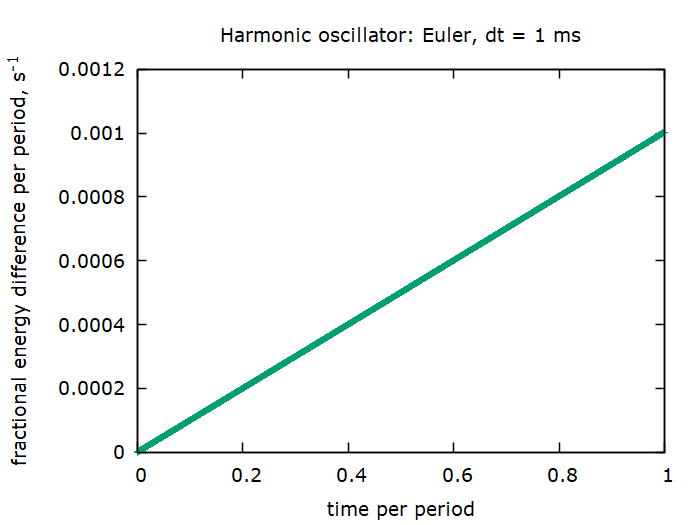
\includegraphics[scale=0.3]{h1.png}
 		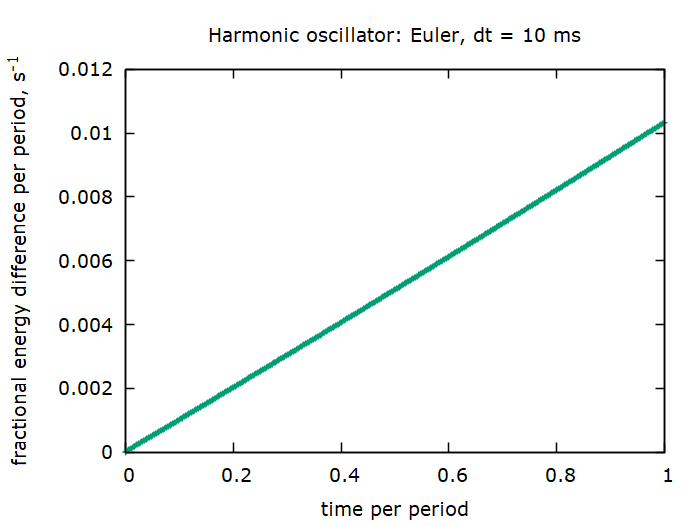
\includegraphics[scale=0.3]{h10.png}
 		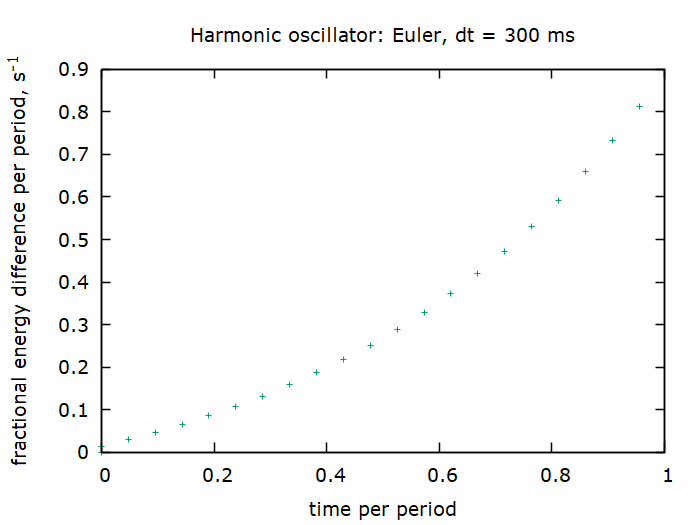
\includegraphics[scale=0.3]{h300.png}
  		\caption{Fractional differences of the calculated energies from the results of Euler's method. At low enough step sizes, the difference is fairly linear through time. We also see that the differences increase by a factor of 10 and then 100 going from $dt = \SI{1}{\mm}$ to $\SI{10}{\mm}$ and $dt = \SI{10}{\mm}$ to $\SI{300}{\mm}$.}
  		\label{gr:hdE}
 	\end{center}
\end{figure}

\begin{figure}[htbp]
  	\begin{center}
 		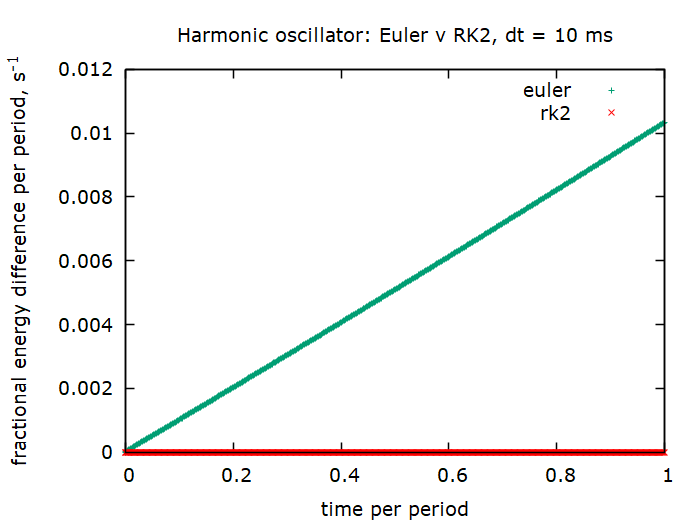
\includegraphics[scale=0.3]{ev2.png}
  		\caption{A comparison of fractional differences in calculated energies from the results of Euler's method and second-order Runge-Kutta method. It is evident that the RK2 method is better than Euler's method in this numerical evaluation, as the RK2 differences look negligible compared to the Euler differences.}
  		\label{gr:ev2}
 	\end{center}
\end{figure}

\begin{figure}[htbp]
  	\begin{center}
 		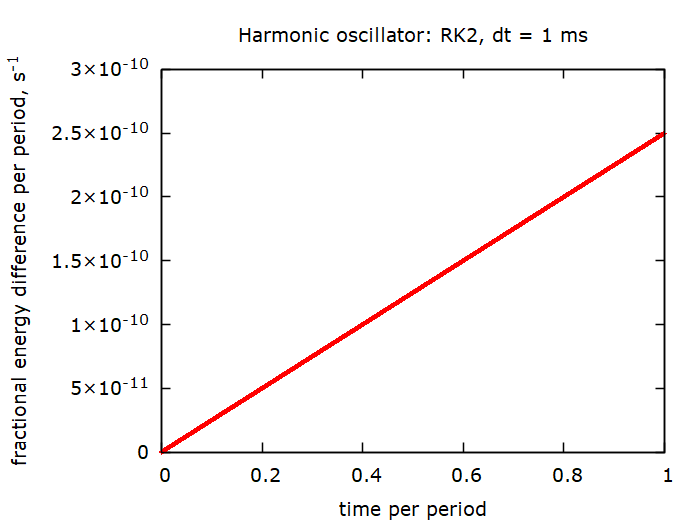
\includegraphics[scale=0.3]{2_1.png}
 		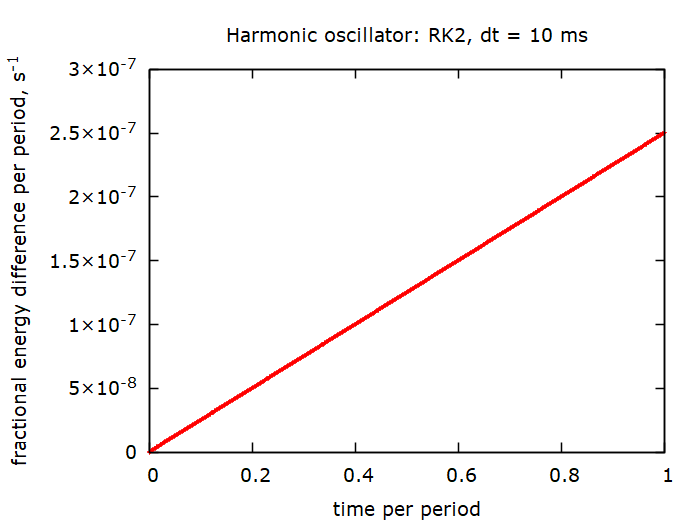
\includegraphics[scale=0.3]{2_10.png}
 		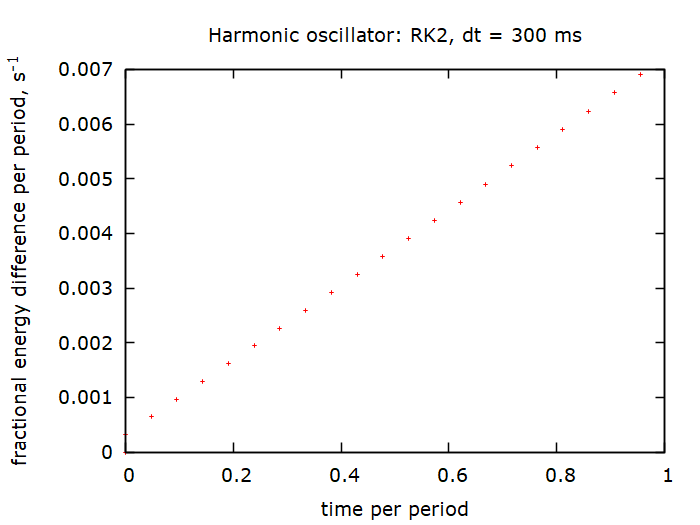
\includegraphics[scale=0.3]{2_300.png}
  		\caption{Similar to Figure \ref{gr:hdE}. We can still see a linear behavior, with the last plot more linear than the last plot for the Euler method results. Also, the change in fractional difference for varying step sizes is more significant for the RK2 method.}
  		\label{gr:rk2dE}
 	\end{center}
\end{figure}

\begin{figure}[htbp]
  	\begin{center}
 		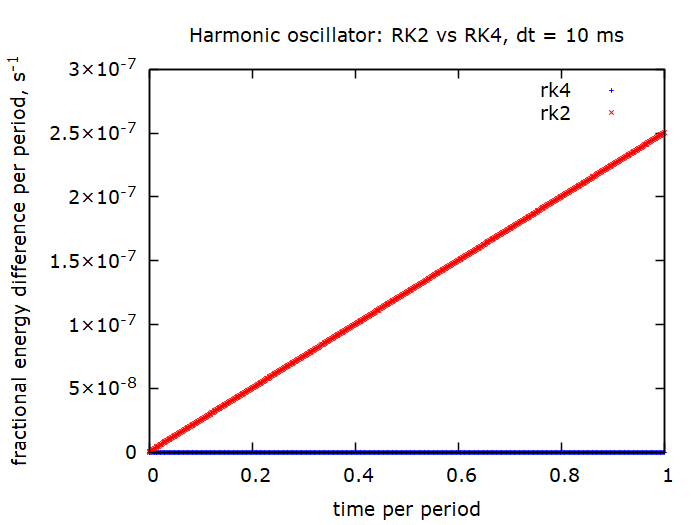
\includegraphics[scale=0.3]{2v4.png}
  		\caption{A comparison of the RK2 and RK4 methods. Like the comparison between Euler and RK2, the RK4 results are negligible relative to the RK2 results, and thus the RK4 method is better.}
  		\label{gr:2v4}
 	\end{center}
\end{figure}

\begin{figure}[htbp]
  	\begin{center}
 		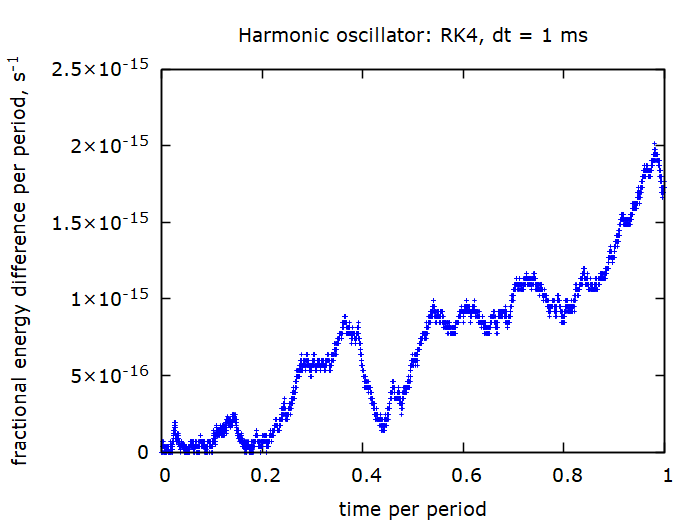
\includegraphics[scale=0.3]{4_1.png}
 		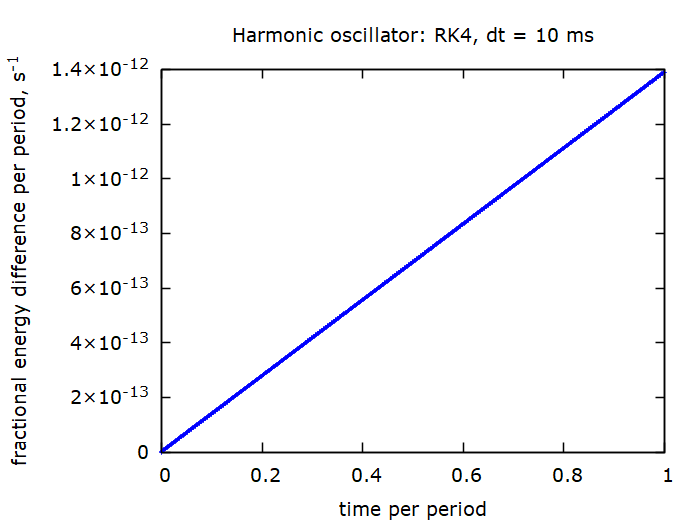
\includegraphics[scale=0.3]{4_10.png}
 		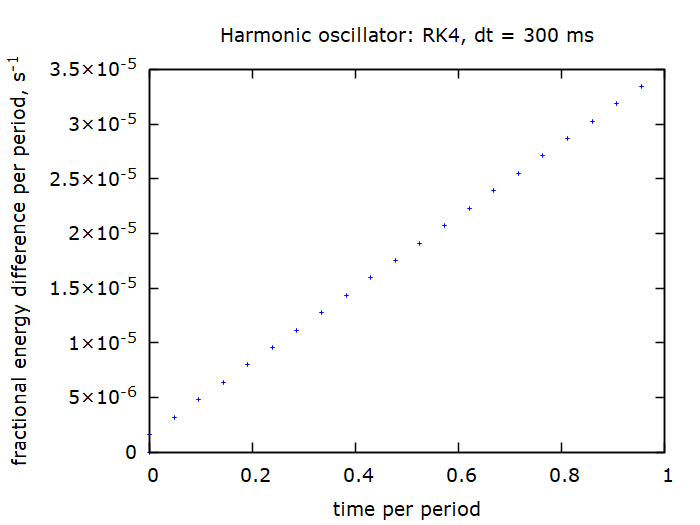
\includegraphics[scale=0.3]{4_300.png}
  		\caption{Similar to Figures \ref{gr:hdE} and \ref{gr:rk2dE}. We get the trend of linear fractional difference for the last two plots, but not for when $dt = \SI{1}{\mm}$. We can see that it is on the order of $10^{-15}$, far less than the results from the other methods, and the differences across varying step sizes are even more significant.}
  		\label{gr:rk4dE}
 	\end{center}
\end{figure}

\subsection{Programming (Mass on a Spring)}
We will need to do an iterative loop over time that will change the values of $x(t)$ and $v(t)$ and recycle the variables by setting them equal to the previous values and putting them back into the loop to get even higher values. For Euler's method, this is straight forward. We can write for the loop,
\begin{lstlisting}
for(t=t0; t<Tmax; t+= dt){
	vt = vtold + dt*(-k/m)*xtold;
	xt = xtold + dt*vtold;
	xtold = xt;  // old -> new
	vtold = vt;
	xtrue = xt0*cos(w*t);
	vtrue = vt0  + -w*sin(w*t);
	Et = 0.5*k*xt*xt + 0.5*m*vt*vt;
	dE = fabs(Et - Etrue)/Etrue;
	// outfile << ... << endl;
}
\end{lstlisting}
For RK2 and RK4 methods, it is slightly more complicated. To make things simple, we will define our correction function in a separate file and call to it in our numerical evaluation. For instance, we can create a file for the RK2 correction which holds the function \cite{RK}
\begin{lstlisting}
double FRK2xv(int ytype, double (*f_x)
(double, double, double), double (*f_v)
(double, double, double), double t,
double xold,double vold,double dt)
{
	double k1x, k1v, k2;
	k1x = dt*(*f_x)(t, xold, vold);
	k1v = dt*(*f_v)(t, xold, vold);
	if(ytype==0){
		k2 = dt*(*f_x)( t, xold+
		k1x/2.0, vold+k1v/2.0 );
	}else{  /* ytype = 1 */
		k2 = dt*(*f_v)( t, xold+
		k1x/2.0, vold+k1v/2.0 );
	}
	return(k2);
\end{lstlisting}
The RK4 method will be exactly the same, but with the higher order terms. Then we can simply implement these into the program for the numerical evaluation as
\begin{lstlisting}
for(t=t0; t<Tmax; t+= dt){
	vt = vtold +
	FRK2xv(1,f_x,f_v,t,xtold,vtold,dt);
	xt = xtold +
	FRK2xv(0,f_x,f_v,t,xtold,vtold,dt);
	xtold = xt;  // old -> new
	vtold = vt;
	...
}
\end{lstlisting}
where we have defined the functions $f_x$ and $f_v$ to be the equations of motion (the subscript indicates which variable is being differentiated).

We are now ready to analyze the results.

\section{Results and Graphs}

\begin{figure}[htbp]
  	\begin{center}
 		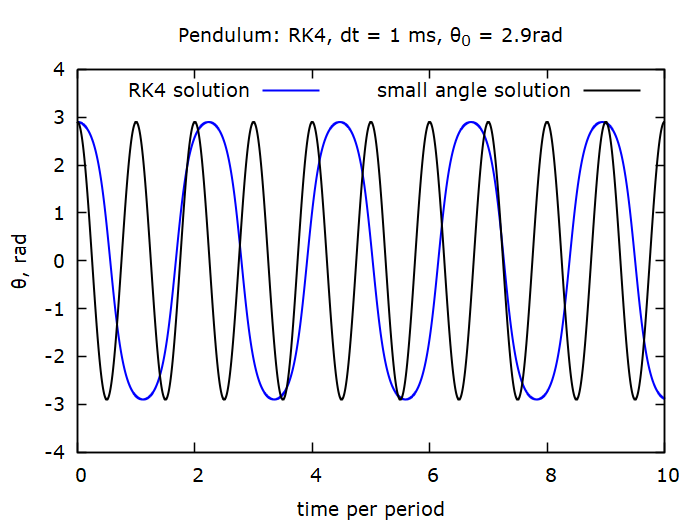
\includegraphics[scale=0.3]{pendfunc.png}
 		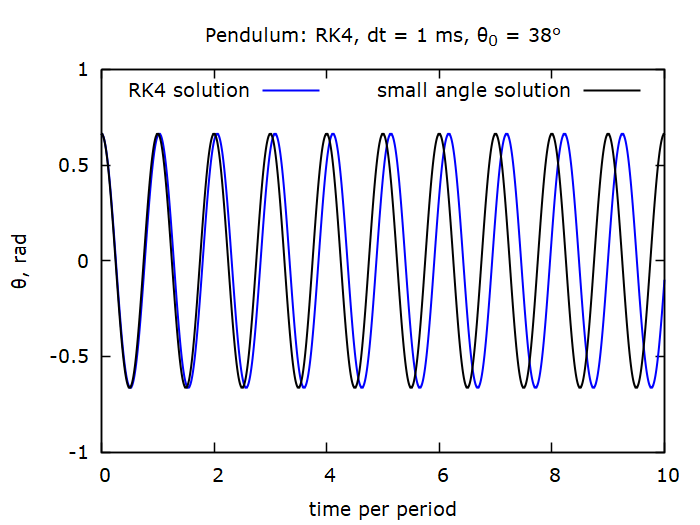
\includegraphics[scale=0.3]{pendfunc38.png}
  		\caption{Comparing the RK4 solution to the 'true' solution using small angle approximation. It is clear that the small angle approximation is very different from the real solution. We can see that the numerical evaluation at smaller angles does begin to converge to an agreement with the small angle approximation solution, but the approximation breaks over time, as we would expect.}
  		\label{gr:pendfunc}
 	\end{center}
\end{figure}

\begin{figure}[htbp]
  	\begin{center}
 		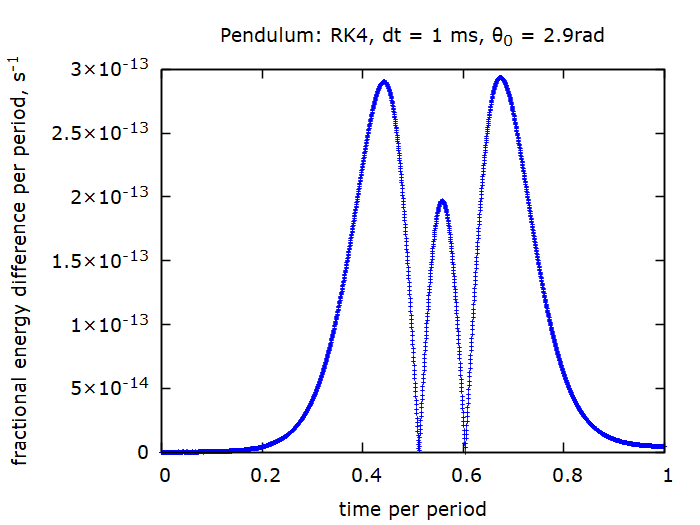
\includegraphics[scale=0.3]{penddE.png}
 		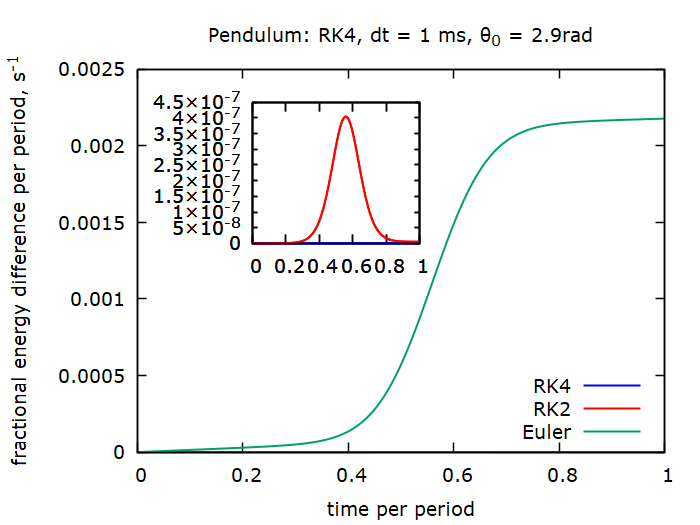
\includegraphics[scale=0.3]{pende24.png}
  		\caption{On top, we can see the fractional energy differences for the pendulum over one period using RK4. We can also see how it compares to the results of the other methods (Euler, RK2) below that. We can see that there is no longer a linear behavior, but more so recognizable and non-fluctuating behavior. The comparison also shows how far the results are from each other, each making the previous negligible.}
  		\label{gr:penddE}
 	\end{center}
\end{figure}

\begin{figure}[htbp]
  	\begin{center}
 		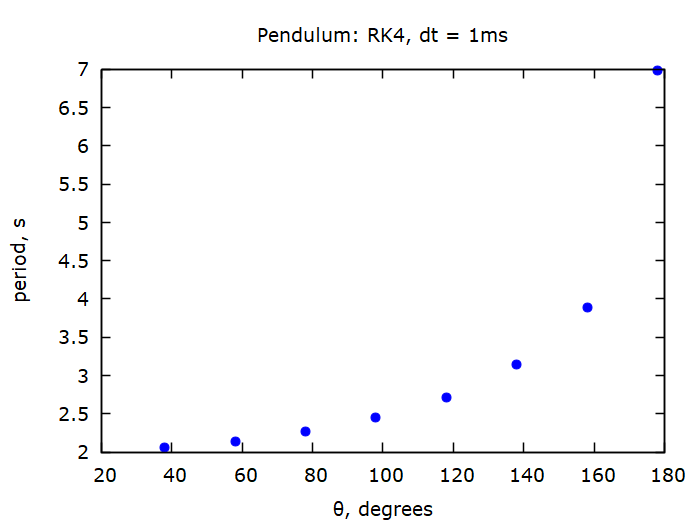
\includegraphics[scale=0.3]{pendthetavT.png}
  		\caption{The period of the $\theta (t)$ functions obtained from the RK4 method for varying starting amplitudes/angle.}
  		\label{gr:pendthetavT}
 	\end{center}
\end{figure}

\section{Discussion and Analysis}

\subsection{Mass on a Spring}
We could numerically approximate the mass on a spring system using Euler's, RK2, and RK4 methods and Figures \ref{gr:hdE} - \ref{gr:rk4dE} show us how they all compare. Immediately, we can see that Euler's method gives agreeing results. Figure \ref{gr:harmosc1} shows just how close the approximation gets to the true solution just at step sizes of $\SI{1}{\ms}$. The fitted values for the frequency and phase of the system are well within $1\sigma$ of the true values. Taking a look at the energy conservation, we see from Figure \ref{gr:hdE} that energy is well conserved at $\SI{1}{\ms}$ and $\SI{10}{\ms}$. It is conserved within a fractional difference of $1$\% per cycle at a maximum step size of about $\SI{9}{\ms}$. For such a simple method of numerical evaluation, this is impressive. But we can also see how larger step sizes break the evaluation. In $\SI{300}{\ms}$ step sizes, the energy is almost at a $100$\% fractional difference after one cycle. This is clearly not good, and it is something we must avoid when performing simulations. Some systems may require extremely small step sizes. Or instead, we can try another method. 
From Figure \ref{gr:ev2}, we can see that the fractional difference in energy from the RK2 results is nothing relative to the Euler results. Figure \ref{gr:rk2dE} reveals that the differences are about one million times smaller for step sizes of $\SI{1}{\ms}$. This is a clear reason why the Runge-Kutta method is favorable over Euler's method. However, we can also see that increasing the step sizes in the same way reveals significant changes in the fractional differences. But even so, at a step size of $\SI{300}{\ms}$, the fractional difference after one cycle is still less than $1$\%. 
This is improved even further using the RK4 method. Figure \ref{gr:2v4} shows that relative to the RK2 results, the RK4 results are negligible. And again, from Figure \ref{gr:rk4dE}, we can see that it yields fractional differences 100000 times smaller at step sizes of $\SI{1}{\ms}$. It may show an even larger jump of $10^{8}$ from $\SI{10}{\ms}$ to $\SI{300}{\ms}$ step sizes, but the fractional difference in energy after one cycle at that large step size is very well below $1$\%, much better than the RK2 result. We do notice some change in behavior from the RK4 results. We could see some pattern of linear behavior from Figures \ref{gr:hdE}, \ref{gr:rk2dE}, and even the last two of Figure \ref{gr:rk4dE}. But the first plot in the RK4 figure fluctuates and is not at all linear. It may be certain 'glitches' pertaining to the calculation or even the capabilities of the computer. The numbers there are so small that precision can easily be lost. We had found before how machine precision can affect the values of our calculations \cite{precision}. It may also be a break in the calculation. Certain values can lead to a certain "error resonance" in recursive approximations like Euler and RK. In any approximation, there are always many values that just do not work for the formula. Since $\SI{10}{\ms}$ and $\SI{300}{\ms}$ showed the expected linear behavior, it may be that $\SI{1}{\ms}$ may be a certain value that breaks RK4. But of course, the fluctuations are so small that actually, we can still use RK4 at such a step size and still achieve accurate results. It is therefore evident that we should use RK4 for the unknown problem, the large amplitude pendulum.

\subsection{Large Amplitude Pendulum}
We can first confirm our results for the known solution at small angles (small angle approximation). From Figure \ref{gr:pendfunc}, the data curve converges towards the true curve as we go to smaller angles. Even at $\SI{38}{\degree}$, the approximation agrees fairly well for the first few cycles, revealing an upper limit for the reliability of the small angle approximation. At larger angles, we can see that the period of the angle oscillation is around two times greater than what the small angle approximation predicts. When we look at the fractional energy differences through time, we see that a step size of $\SI{1}{\ms}$ gives a non linear behavior in all of the approximation methods. This may show that the 'outliar' behavior in Figure \ref{gr:rk4dE} may not be an error in calculation, but more so an underlying behavior of the actual function. The behaviors in Figure \ref{gr:penddE} are not chaotic. I do not know what is the underlying cause of this. It may be due to the functions of $\theta (t)$ and $\omega (t)$ in the equation for energy creating a superposition of sinusoidal waves. Whatever the case, it is clear how small the fractional differences are compared to each method, with the Euler method showing the greatest difference, but still much less than $1$\%.
If we take a look at how the period of the pendulum varies as a function of the angle in Figure \ref{gr:pendthetavT}, we can see that there is definitely a relationship between the angle and the period. This is not what we would expect if we used small angle approximation for all angles. We would instead predict that there is no relationship. But from the figure, we can confirm that at smaller angles, which we can quantify is around $\SI{40}{\degree}$ by reading off the curve, there is a constant behavior. Recall that these results are assuming a model of a massless rod holding the pendulum bob, otherwise at such large angles, the mass would fall straight down with a behavior not described by the equations of motions we used. Then it makes sense that the period behaves like we see in the figure. As the angle approaches 0, the period should also approach 0. And as the angle gets closer to $\SI{180}{\degree}$, the period should get longer and longer, as gravity will fight the normal force of the rod, resulting in slower accelerations in the beginning, which approaches infinity (i.e. the rod stands straight up at $\SI{180}{\degree}$ forever). 

\section{Conclusions}
The Euler and Runge-Kutta methods have proven to both be useful tools in solving differential equations numerically. We found that the RK method worked better, but of course, it relies on the techniques employed by the Euler method. Applying both of these to a system we knew the solution to revealed the behaviors that may come up when doing a numerical evaluation over an analytic one. We are going to get error inevitably by using approximations, we can find how changing our step size can reduce that error. And once we understood how the numerical methods applied to the known system, we could apply it to a system with an unknown analytic solution and discover some behaviors that we may have otherwise not predicted. This has proven to show the capabilities of computational methods. With fairly simple mathematical techniques, we can discover the behaviors of multiple types of systems so long as we can first find the equations of motion.
\section*{Acknowledgments}
\setlength{\parindent}{0cm}

\bibliographystyle{aipauth4-1}
\bibliography{bib7}



\end{document}